% $> xelatex presentacion.tex
% o bien
% $> lualatex presentacion.tex
\documentclass[spanish]{beamer}

\usepackage[es-tabla]{babel}

\usepackage{graphics,tikz}
\usetikzlibrary{automata, positioning, arrows}

\usepackage{adjustbox}
\usepackage{booktabs}
\usepackage{multirow}
\usepackage{enumitem}

%%% FUENTES

\usepackage[no-math]{fontspec}
\setmainfont{Libertinus Serif}
\setsansfont{Libertinus Sans}
\setmonofont{Libertinus Mono}

\usepackage{pifont}
\newcommand{\cmark}{\ding{51}}%
\newcommand{\xmark}{\ding{55}}%

%%% COLORES

\definecolor{background}{HTML}{FFFFFF}
\definecolor{foreground}{HTML}{3F3F3F}
\definecolor{strings}{HTML}{ED982C}
\definecolor{operators}{HTML}{CF4818}
\definecolor{identifiers}{HTML}{9A71BA}
\definecolor{keywords}{HTML}{5486C8}
\definecolor{numbers}{HTML}{80951D}
\definecolor{comments}{HTML}{AFAFAF}

%%% LISTINGS

\usepackage{listings}

\lstset{
  numbers=left,
  belowcaptionskip=1\baselineskip,
  basicstyle=\scriptsize\ttfamily\color{foreground},
  keywordstyle=\color{keywords},
  commentstyle=\color{comments},
  stringstyle=\color{strings},
  identifierstyle=\color{identifiers},
  numberstyle=\color{foreground},
  xleftmargin=2em,
  framexleftmargin=1.5em,
  breaklines=true,
  showstringspaces=false,
  tabsize=2
}


%%% AJUSTES DE BEAMER

%\usefonttheme{professionalfonts}

\setlength{\leftmargini}{0cm}
\setlength{\leftmarginii}{2em}

\setbeamertemplate{navigation symbols}{}

\setbeamerfont{title}{series=\bfseries}

%\setbeamertemplate{frametitle}{\color{foreground}\vspace*{1cm}\bfseries\insertframetitle\par\vskip-6pt}
\setbeamerfont{frametitle}{series=\bfseries}
\setbeamercolor{frametitle}{fg=foreground}
\setbeamerfont{framesubtitle}{size=\normalfont\small}
\setbeamercolor{framesubtitle}{fg=foreground}

\setbeamercolor{background canvas}{bg=background}

\setbeamercolor{normal text}{fg=foreground}
\setbeamercolor{alerted text}{fg=foreground}
\setbeamercolor{block title}{fg=foreground}
\setbeamercolor{alerted text}{fg=foreground}

\setbeamercolor{itemize item}{fg=foreground}
\setbeamercolor{enumerate item}{fg=foreground}

\setbeamertemplate{itemize items}[circle]
\setitemize{
  label=\usebeamerfont*{itemize item}
  \usebeamercolor[fg]{itemize item}
  \usebeamertemplate{itemize item}
}

\setbeamercolor*{title}{fg=foreground}
\setbeamercolor{qed symbol}{fg=foreground}

\usebeamercolor[fg]{normal text}

\setbeamertemplate{footline}{
    \hbox{%
    \begin{beamercolorbox}[wd=\paperwidth,ht=3ex,dp=1.5ex,leftskip=2ex,rightskip=2ex]{page footer}%
        \usebeamerfont{title in head/foot}%
            \insertsection \hfill
        \insertframenumber{} / \inserttotalframenumber
    \end{beamercolorbox}}%
}
\setbeamerfont{footline}{size=\fontsize{9}{11}\selectfont}

\setbeamercolor{section in toc}{fg=foreground}
\setbeamerfont{section in toc}{series=\bfseries}

\setbeamercolor{caption name}{fg=foreground}
\setbeamerfont{caption name}{series=\bfseries}

\setbeamercolor{bibliography entry note}{fg=foreground}
\setbeamercolor{bibliography entry author}{fg=foreground!40!black}

\hypersetup{
  colorlinks=true,
  citecolor=numbers,
  urlcolor=operators,
  linkcolor=foreground
}

%%% INFORMACIÓN DEL DOCUMENTO

\title{Generación de música mediante redes neuronales profundas}
\subtitle{Trabajo de fin de grado}
\author{Antonio Martín Ruiz}
\institute{\normalsize Universidad de Granada}
\date{17 de septiembre de 2020\texorpdfstring{\\}{} \small Curso 2019-2020}

\begin{document}

\maketitle

\begin{frame}{Índice}
\tableofcontents
\end{frame}

\section{Aprendizaje profundo}

\begin{frame}{Redes neuronales profundas}

$$f^*(\mathbf{x}) \approx f(\mathbf{x}; \theta) = (f_1 \circ f_2 \circ ... \circ f_N)(\mathbf{x}) $$

$$f_i(\mathbf{x};\mathbf{W}_i,\mathbf{b}_i) = \sigma(\mathbf{W}_i^T\mathbf{x} + \mathbf{b}_i)$$
\begin{figure}
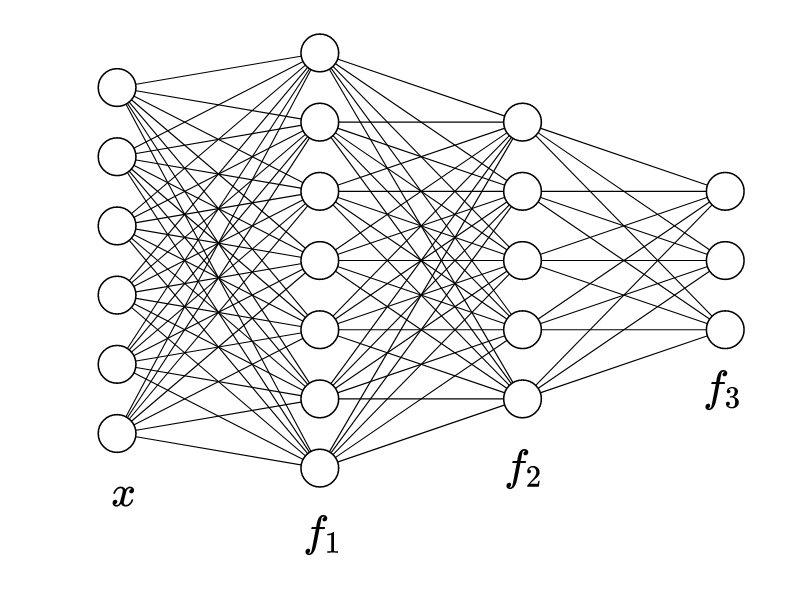
\includegraphics[scale=0.20]{img/nn1.png}
\caption{Ejemplo de red neuronal prealimentada con dos capas ocultas}
\end{figure}

\end{frame}

\section{Aproximación por superposición de funciones sigmoidales}

\begin{frame}{Teorema de Hahn Banach}

\textit{Teorema de extensión de Hahn-Banach}. $X$ espacio normado, $M$ subespacio de $X$, $g \in M^*$ entonces $\exists$ $f \in X^*$ que extiende a $g$ con $\Vert f \Vert = \Vert g \Vert$.
\\~\

\pause

\textit{Corolario}. $X$ espacio normado, $M$ un subespacio de $X$. Si $x_0 \notin \overline{M}$, $\exists$ $f \in X^*$ tal que $f(x) = 0$ $\forall x \in M$, $f(x_0) = 1$, y $\Vert f \Vert = \frac{1}{d}$, donde $d$ es la distancia de $x_0$ a $M$.

\pause

\textit{Demostración}. $y = x + ax_0$. $f(x+ax_0) = a$ lineal, $\Vert f \Vert = \frac{1}{d}$. Aplicar extensión.
\end{frame}

\begin{frame}{Teorema de representación de Riesz}

\textit{Teorema}. $X$ un espacio de Hausdorff localmente compacto, $T$ funcional lineal acotado sobre $C_0(X)$. $\exists$ $\mathcal{M}$ $\sigma$-álgebra en $X$ que contiene todos los conjuntos de Borel en $X$ y $\exists !$ $\mu$ medida con signo regular sobre $\mathcal{M}$ tal que $$ T(f) = \int_X fd\mu$$ para cada $f \in C_0(X)$. Además $$\Vert T \Vert = \vert \mu \vert (X).$$
\end{frame}

\begin{frame}{Teorema para funciones discriminatorias}

\textit{Definición}. $\sigma: \mathbb{R} \rightarrow \mathbb{R}$ es \textit{discriminatoria} si, cuando para una medida $\mu \in M(I^n)$ se tiene que $$\int_{I^n} \sigma(\textbf{y}^T \textbf{x} + \theta)d\mu(\textbf{x})= 0$$
para todo $\textbf{y} \in \mathbb{R}^n$, $\theta \in \mathbb{R}$ implica que $\mu = 0$.
\\~\

\pause

\textit{Teorema}. $\sigma$ continua discriminatoria. Entonces
$$S = \left\{ g: g(\textbf{x}) = \sum_{j=1}^k \alpha_j \sigma(\textbf{y}_j^T \textbf{x} + \theta_j) \right\}$$
es denso en $C(I^n)$.
\pause

\textit{Demostración}. Si $\overline{S} \neq C(I^n)$, aplicar corolario de H-B para obtener funcional, que por Riezs es $F(h) = \int_{I^n}h(\textbf{x})d\mu(\textbf{x})$, nulo. Contradicción.

\end{frame}

\begin{frame}{Lema de funciones sigmoidales}
\textit{Lema}. Las funciones sigmoidales continuas son discriminatorias.

\pause
\textit{Demostración}.
$$\sigma (\lambda (\textbf{y}^T\textbf{x} + \theta) + \phi) \left\{ \begin{array}{lclcc}
             \rightarrow 1 &   si  & \textbf{y}^T\textbf{x} + \theta > 0 $ cuando $ \lambda \rightarrow + \infty,
             \\ \rightarrow 0 &   si & \textbf{y}^T\textbf{x} + \theta < 0 $ cuando $ \lambda \rightarrow + \infty,
             \\ = \sigma(\phi) &   si & \textbf{y}^T\textbf{x} + \theta = 0 $ para todo $ \lambda.
             \end{array}
   \right.$$

converge puntualmente a

$$\gamma(\textbf{x})= \left\{ \begin{array}{lcl}
             1 &   si  & \textbf{y}^T\textbf{x} + \theta > 0
             \\ 0 &   si & \textbf{y}^T\textbf{x} + \theta < 0
             \\ \sigma(\phi) &   si & \textbf{y}^T\textbf{x} + \theta = 0
             \end{array}
   \right.$$

Por convergencia dominada, $$0 =  \lim_{\lambda \rightarrow \infty}\int_{I^n} \sigma(\lambda(\textbf{y}^T\textbf{x} + \theta) + \phi)d\mu(\textbf{x}) = \sigma(\phi)\mu(\Pi_{\textbf{y}, \theta}) + \mu(H_{\textbf{y}, \theta})$$
\end{frame}

\begin{frame}
$$F(h) = \int_{I^n}h(\textbf{y}^T\textbf{x})d\mu(\textbf{x}), h \in L^{\infty}(\mathbb{R})$$

Tomando $h$ función indicadora en $[\theta, +\infty)$.
$$F(h) = \int_{I^n}h(\textbf{y}^T\textbf{x})d\mu(\textbf{x}) = \mu(\Pi_{\textbf{y}, -\theta}) + \mu(H_{\textbf{y}, -\theta}) = 0 \Rightarrow F = 0$$

Tomando $s(u) = \sin(m \cdot u)$, $c(u) = \cos(m \cdot u)$,

$$F(s + ic) = \int_{I^n}(\cos(m^Tx) + i \sin(m^Tx))d\mu(x) = \int_{I^n}exp(im^Tx)d\mu(x) = 0$$ $$\Rightarrow \mu = 0$$

\end{frame}

\begin{frame}{Teorema para funciones sigmoidales}
\textit{Teorema}. $\sigma$ sigmoidal continua. Entonces
$$S = \left\{ g: g(\textbf{x}) = \sum_{j=1}^k \alpha_j \sigma(\textbf{y}_j^T \textbf{x} + \theta_j) \right\}$$
es denso en $C(I^n)$.

\end{frame}

\begin{frame}{Otros resultados}

\begin{itemize}
\item Generalización para funciones acotadas no constantes.
\item Generalización para funciones Riemann-integrables no polinomiales.
\item Anchura fija y profundidad arbitraria.
\end{itemize}

\end{frame}

\section{Tratamiento de secuencias}

\begin{frame}{Redes neuronales recurrentes}

\begin{figure}
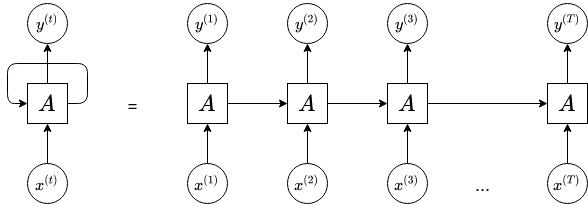
\includegraphics[scale=0.5]{img/recurrent.png}
\caption{Desenrollado de una red recurrente}
\end{figure}

\end{frame}

\begin{frame}{Redes recurrentes bidireccionales y profundas}

\begin{figure}
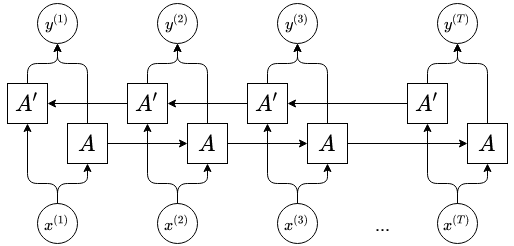
\includegraphics[scale=0.5]{img/bidirectional.png}
\caption{Red recurrente bidireccional}
\end{figure}

\end{frame}

\begin{frame}{Redes recurrentes con puertas}

\begin{figure}
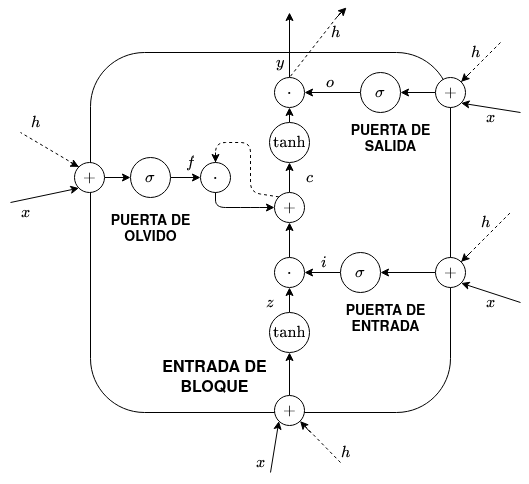
\includegraphics[scale=0.41]{img/LSTM.png}
\caption{Bloque LSTM (Long short-term memory)}
\end{figure}

\end{frame}

\section{Aprendizaje de características}

\begin{frame}{Autoencoder}

\begin{figure}
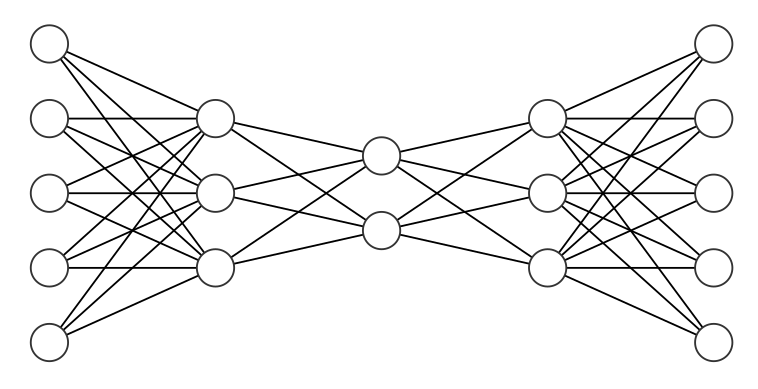
\includegraphics[scale=0.4]{img/autoencoder.png}
\caption{Estructura de un \textit{autoencoder} como red prealimentada profunda}
\end{figure}

\end{frame}

\begin{frame}{Autoencoder variacional}

$$ p_{\boldsymbol{\theta}}(\textbf{z}|\textbf{x}) = \frac{p_{\boldsymbol{\theta}}(\textbf{x}|\textbf{z})p_{\boldsymbol{\theta}}(\textbf{z})}{p_{\boldsymbol{\theta}}(\textbf{x})}$$

$$p_{\theta}(\textbf{z} \vert \textbf{x}) \approx q_{\phi}(\textbf{z} \vert \textbf{x}) = \mathcal{N}(\textbf{x};\boldsymbol{\mu}, \boldsymbol{\sigma}^2\textbf{I}) $$

\begin{figure}
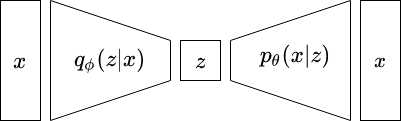
\includegraphics[scale=0.6]{img/vae.png}
\caption{Estructura de un \textit{autoencoder} variacional}
\end{figure}

\end{frame}

\begin{frame}{Función de coste del VAE}

\textit{Definición.} P y Q distribuciones sobre el mismo espacio de probabilidad, se define la divergencia de Kullback-Leibler como

$$D_{KL}(Q \parallel P) = E_Q \left[ \log \frac{Q(x)}{P(x)} \right].$$
\\~\

\textit{Proposición. } Dadas las distribuciones de probabilidad  $p(\textbf{x}) = N(\textbf{x};\boldsymbol{\mu}_1, \boldsymbol{\Sigma}_1) $ y $q(\textbf{x}) = N(\textbf{x};\boldsymbol{\mu}_2, \boldsymbol{\Sigma}_2)$, ambas de dimensión $k$,
se cumple que $D_{KL}(p(\textbf{x}) \parallel q(\textbf{x})) = \frac{1}{2} \left( \log \frac{|\boldsymbol{\Sigma}_1|}{|\boldsymbol{\Sigma}_2|} - k + tr(\boldsymbol{\Sigma}_2^{-1}\boldsymbol{\Sigma}_1) + (\boldsymbol{\mu}_2 - \boldsymbol{\mu}_1)^T \boldsymbol{\Sigma}_2^{-1} (\boldsymbol{\mu}_2 - \boldsymbol{\mu}_1) \right)$.
\end{frame}

\begin{frame}{Cálculo de ELBO (Evidente lower bound)}

$$D_{KL}(q_{\boldsymbol{\phi}}(\textbf{z}|\textbf{x}) \parallel p_{\boldsymbol{\theta}}(\textbf{z}|\textbf{x})) =$$ $$ E_{z \sim q_{\boldsymbol{\phi}} (\textbf{z}|\textbf{x})} \left[ \log q_{\boldsymbol{\phi}}(\textbf{z}|\textbf{x}) - \log p_{\boldsymbol{\theta}}(\textbf{z}|\textbf{x}) \right] =$$

\pause
$$E_{z \sim q_{\boldsymbol{\phi}} (\textbf{z}|\textbf{x})} \left[ \log q_{\boldsymbol{\phi}}(\textbf{z}|\textbf{x}) - \log  \frac{p_{\boldsymbol{\theta}}(\textbf{x}|\textbf{z})p_{\boldsymbol{\theta}}(\textbf{z})}{p_{\boldsymbol{\theta}}(\textbf{x})}\right]=$$ $$ E_{z \sim q_{\boldsymbol{\phi}} (\textbf{z}|\textbf{x})} \left[ \log q_{\boldsymbol{\phi}}(\textbf{z}|\textbf{x}) - \log  p_{\boldsymbol{\theta}}(\textbf{x}|\textbf{z}) - \log p_{\boldsymbol{\theta}}(\textbf{z}) + \log p_{\boldsymbol{\theta}}(\textbf{x})\right].$$

\pause
$$ D_{KL}(q_{\boldsymbol{\phi}}(\textbf{z}|\textbf{x}) \parallel p_{\boldsymbol{\theta}}(\textbf{z}|\textbf{x})) - \log p_{\boldsymbol{\theta}}(\textbf{x}) =$$ $$ E_{z \sim q_{\boldsymbol{\phi}} (\textbf{z}|\textbf{x})} \left[ \log q_{\boldsymbol{\phi}}(\textbf{z}|\textbf{x}) - \log  p_{\boldsymbol{\theta}}(\textbf{x}|\textbf{z}) - \log p_{\boldsymbol{\theta}}(\textbf{z})\right] = $$

\pause
$$ - E_{z \sim q_{\boldsymbol{\phi}} (\textbf{z}|\textbf{x})} \left[ \log p_{\boldsymbol{\theta}}(\textbf{x}|\textbf{z}) \right] + E_{z \sim q_{\boldsymbol{\phi}} (\textbf{z}|\textbf{x})} \left[ \log  q_{\boldsymbol{\phi}}(\textbf{z}|\textbf{x}) - \log p_{\boldsymbol{\theta}}(\textbf{z})\right]=$$ $$ - E_{z \sim q_{\boldsymbol{\phi}} (\textbf{z}|\textbf{x})} \left[ \log p_{\boldsymbol{\theta}}(\textbf{x}|\textbf{z}) \right] + D_{KL}(q_{\boldsymbol{\phi}}(\textbf{z}|\textbf{x}) \parallel p_{\boldsymbol{\theta}}(\textbf{z})).$$

\end{frame}

\begin{frame}{Truco de reparametrización}

$$L(\boldsymbol{\theta}, \boldsymbol{\phi}; \textbf{x}) = - E_{z \sim q_{\boldsymbol{\phi}} (\textbf{z}|\textbf{x})} \left[ \log p_{\boldsymbol{\theta}}(\textbf{x}|\textbf{z}) \right] +  \frac{1}{2}\sum_{j=1}^k \left( -log(\sigma_j^2) -1 + \sigma_j^2 + \mu_j^2 \right). $$

$$\tilde{L}(\boldsymbol{\theta}, \boldsymbol{\phi}; \textbf{x}) = -\frac{1}{\mathcal{L}}\sum_{l=1}^{\mathcal{L}}\log p_{\boldsymbol{\theta}}(\textbf{x}^{(i)}|\textbf{z}^{(i,l)}) +  \frac{1}{2}\sum_{j=1}^k \left( -log(\sigma_j^2) -1 + \sigma_j^2 + \mu_j^2 \right).$$

\end{frame}

\section{MusicVAE}

\begin{frame}{MusicVAE}

\begin{figure}
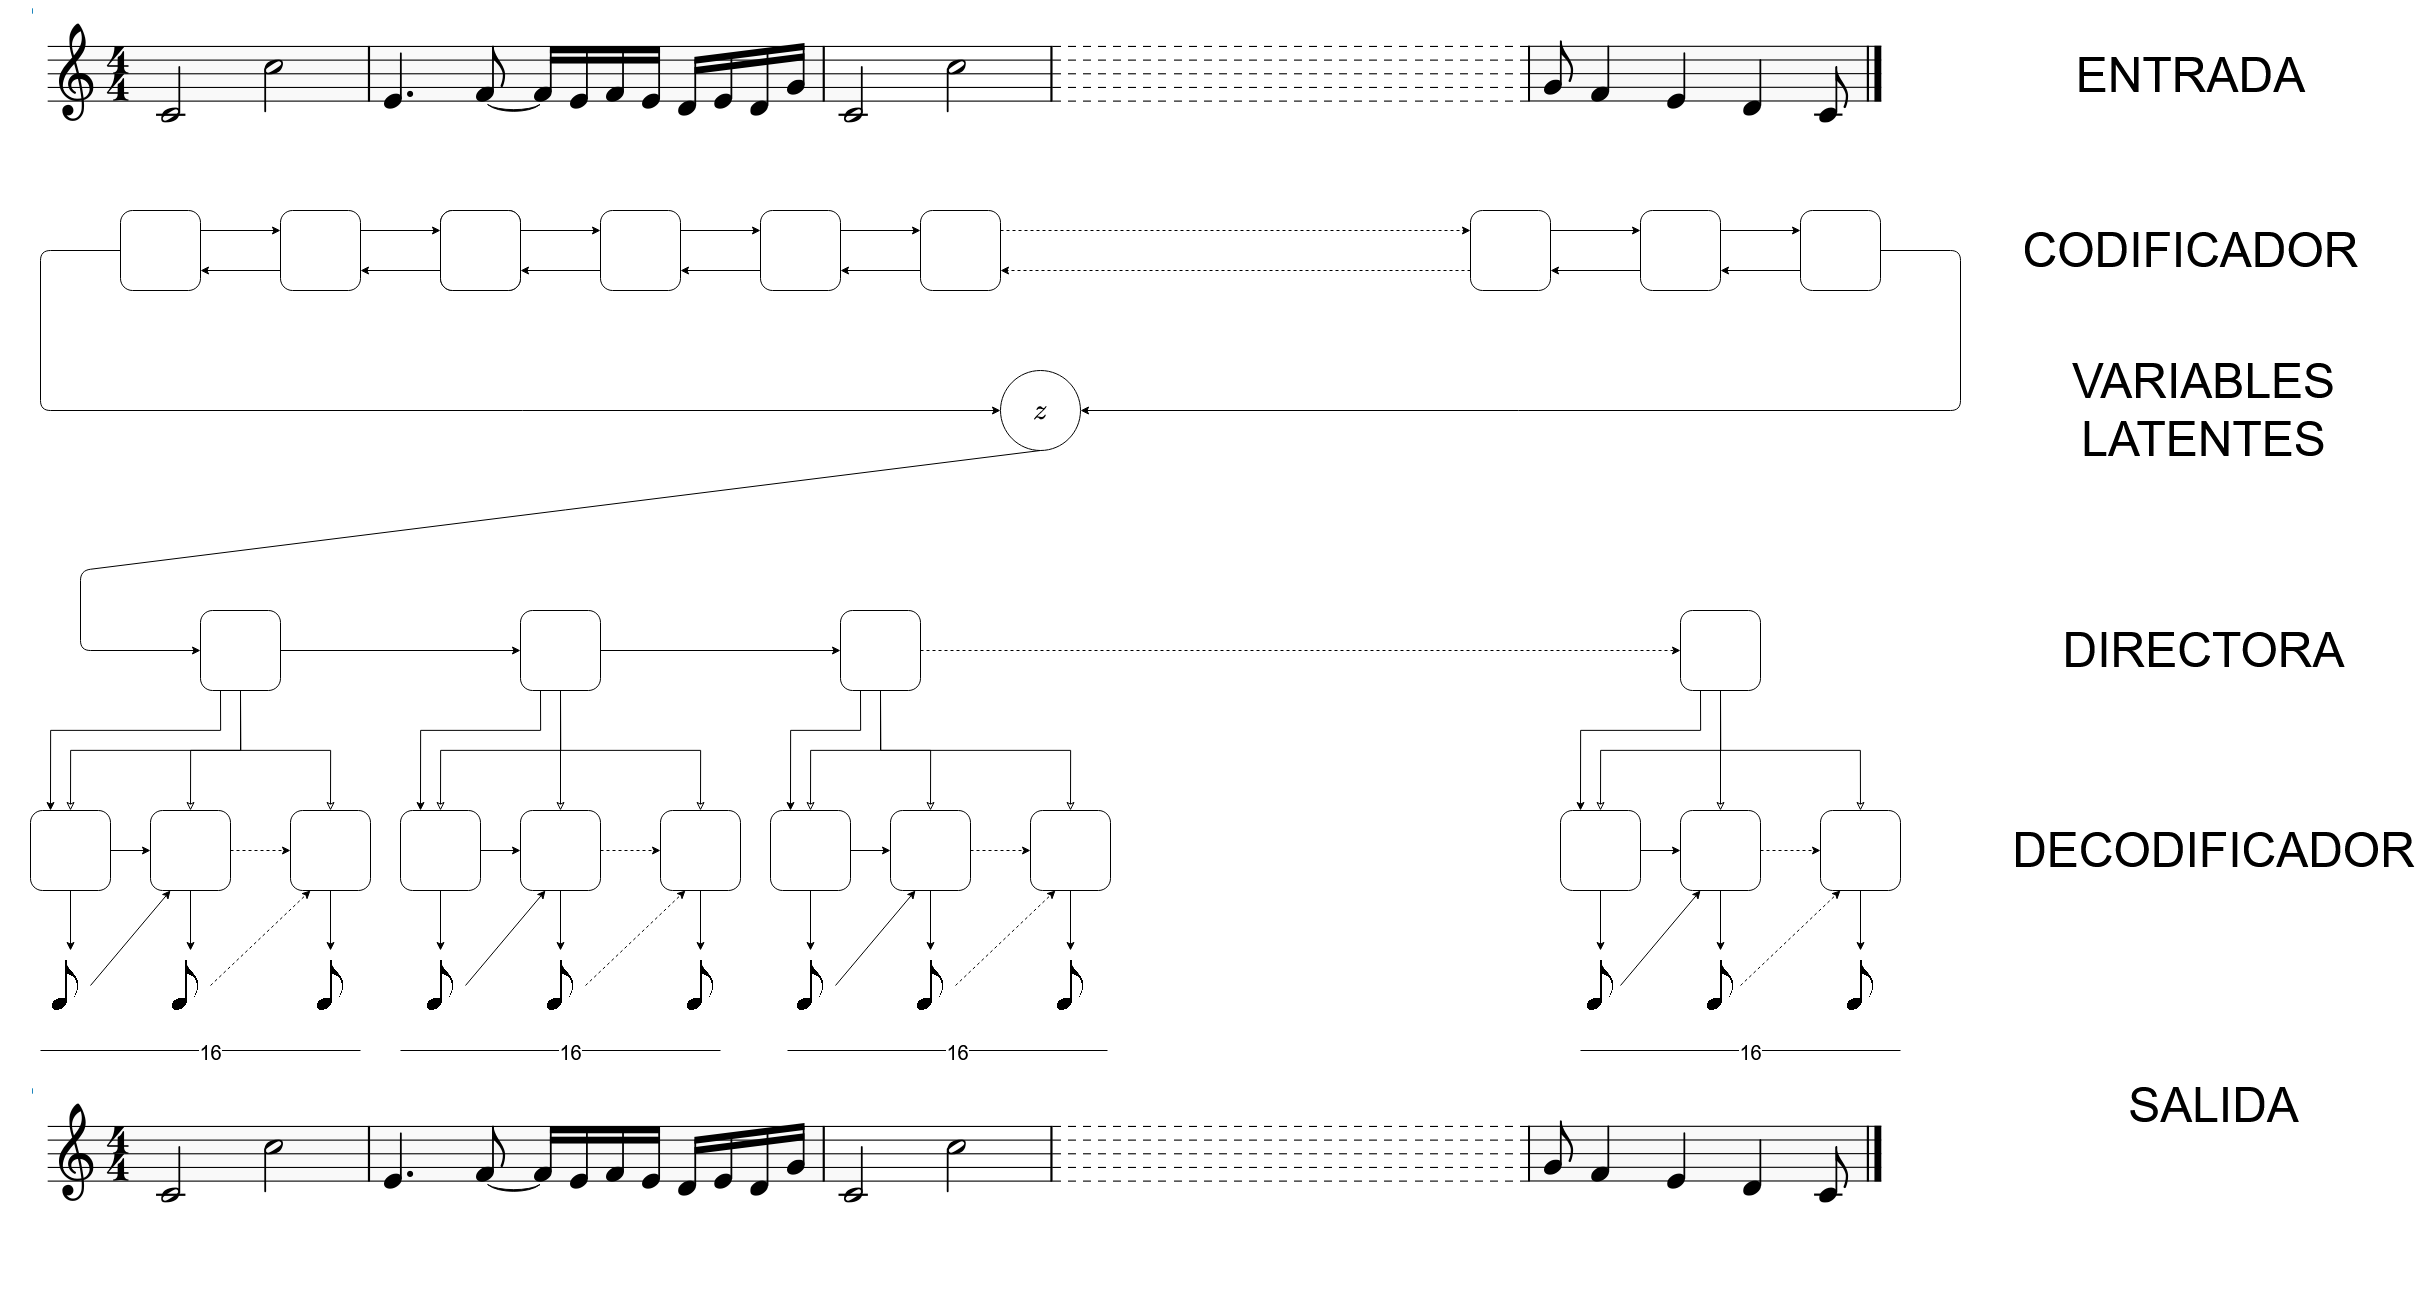
\includegraphics[scale=0.16]{img/musicvae.png}
\caption{Estructura del modelo MusicVAE}
\end{figure}


\end{frame}

\section{AutoLoops}

\begin{frame}{AutoLoops}
\end{frame}

\end{document}
